\documentclass[12pt,a4paper]{article}

\usepackage[utf8]{inputenc}
\usepackage[T1]{fontenc}
\usepackage[english]{babel}
\usepackage[margin=2.5cm]{geometry}
\usepackage{graphicx}
\usepackage{fancyhdr}
\usepackage{hyperref}
\usepackage{enumitem}
\usepackage{lastpage}
\usepackage{titlesec}
\usepackage{setspace}

\hypersetup{
  colorlinks=true,
  linkcolor=black,
  urlcolor=blue,
  citecolor=black,
  pdfauthor={Pedro Castro},
  pdftitle={Bomberman}
}

\graphicspath{{images/}}

\pagestyle{fancy}
\fancyhf{}
\rfoot{\small \thepage\ /\ \pageref{LastPage}}
\renewcommand{\headrulewidth}{0pt}

\titlespacing*{\section}{0pt}{1.5\baselineskip}{0.5\baselineskip}
\titlespacing*{\subsection}{0pt}{1\baselineskip}{0.25\baselineskip}

\onehalfspacing%

\newcommand{\coverpage}[4]{
  \begin{titlepage}
    \centering
    \vspace*{1.5cm}

    {\bfseries\Large Faculty of Engineering — University of Porto}\\[1.5cm]

    
\includegraphics[width=0.5\textwidth]{feup.png}\\[1.5cm]

    {\Huge \bfseries #1}\\[1cm]

    \if\relax\detokenize{#2}\relax\else
      {\Large #2}\\[1cm]
    \fi

    \vspace*{\fill}
    \if\relax\detokenize{#3}\relax\else
      \includegraphics[width=0.5\textwidth]{#3}
    \fi
    \vspace*{\fill}

    {\large\bfseries\begin{tabular}{c} #4 \end{tabular}}\\[1cm]

    {\large \today}

    \vspace*{1cm}
  \end{titlepage}
}

\begin{document}

\coverpage%
  {Bomberman}
  {A Bomberman clone built in C for MINIX-LCOM.}
  {logo.png}
  {Nuno Gomes\\Pedro Castro\\Vasco Lemos}

\clearpage
\tableofcontents
\clearpage

\section{Project Goal and Description}
What was our goal? What is our application?

\section{Architecture and Structure}

Our project implements a Model-View-Controller (MVC) architecture, providing separation of concerns and maintainable code organization. The architecture is divided into three main components, each with specific responsibilities and well-defined communication patterns.

\begin{figure}[ht]
  \centering
  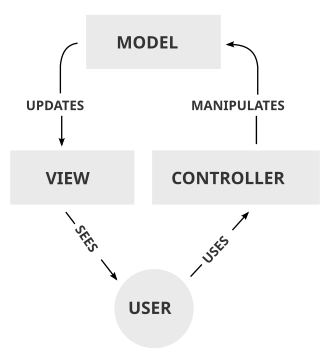
\includegraphics[width=1.0\textwidth]{architecture.png}
  \caption{System architecture diagram.}\label{fig:architecture}
\end{figure}

\subsection{Model Component}

The Model component manages the game's core data structures and business logic, organized into several modules:

\begin{itemize}[itemsep=0.5em]
  \item \textbf{Game:} Central component that maintains the overall game state, including current game state, score, level progression, and timer management. The \texttt{Game} struct serves as the primary data container for all game entities.
  \item \textbf{Entity:} Defines the base \texttt{Entity} structure used for all game objects (player, enemies, bombs, walls, bricks). Provides common functionality such as position management, sprite handling, and movement.
  \item \textbf{Board:} Handles maze parsing from text files and maintains the spatial representation of the game maze. Manages different board elements and provides the foundation for collision detection.
  \item \textbf{Sprite:} Manages sprite creation from XPM files and animated sprites for dynamic entities. Handles sprite rendering and animation frame updates.
  \item \textbf{Resources:} Centralizes asset management by loading and storing all game sprites, ensuring efficient memory usage and providing a single access point for graphical resources.
\end{itemize}

\subsection{View Component}

The View component is responsible for all rendering operations and visual presentation:

\begin{itemize}[itemsep=0.5em]
  \item \textbf{Rendering:} Implements frame caching to optimize performance, drawing different screens based on game state (start menu, pause menu, game screen, win/lose screens).
  \item \textbf{Game Visualization:} Renders the game board, all entities, user interface elements (score, lives, timer), and provides visual feedback for player interactions.
  \item \textbf{Menu System:} Handles drawing of interactive menus with mouse hover highlighting and button states.
\end{itemize}

\subsection{Controller Component}

The Controller component manages input handling and system-level operations:

\begin{itemize}[itemsep=0.5em]
  \item \textbf{Device Drivers:} Low-level modules for timer, keyboard, mouse, graphics and RTC hardware, providing hardware abstraction.
  \item \textbf{Interrupt Handlers:} Coordinates all hardware interrupt subscriptions and delegates interrupt processing to appropriate handlers.
  \item \textbf{Input Module:} Abstracts keyboard input by converting scan codes into logical key representations (KEY\_UP, KEY\_DOWN, etc.) and defines interaction areas for menu navigation.
  \item \textbf{Event Handlers:} Processes high-level game events from keyboard, mouse, timer, and RTC interrupts. Translates raw input into meaningful game actions and state changes.
\end{itemize}

\subsection{Communication Patterns}

The MVC components communicate through well-defined interfaces:

\textbf{Controller $\rightarrow$ Model:} Hardware interrupts are processed by interrupt handlers, which call event handlers that modify the game state. For example, keyboard events trigger player movement by calling movement functions that update entity positions in the game model.

\textbf{Model $\rightarrow$ View:} The view component receives the current game state and renders the appropriate visual representation. The \texttt{draw\_next\_frame()} function determines which screen to display based on the game's current state.

\textbf{Main Loop:} The main game loop in \texttt{proj.c} orchestrates the entire system by receiving hardware interrupts, processing them through the controller, updating the model, and triggering view updates. This event-driven architecture ensures a clear separation of concerns.

The architecture's modularity allows for easy maintenance and extension, with each component handling its specific responsibilities while maintaining loose coupling through well-defined interfaces.

\section{Devices and Interfaces Used}
What devices did we use and for what purpose?
\begin{itemize}[itemsep=0.5em]
  \item \textbf{Mouse:} \ldots
  \item \textbf{Timer:} \ldots
  \item \textbf{Keyboard:} \ldots
  \item \textbf{RTC:} \ldots
\end{itemize}

\section{Differentiating Features}
What are the differentiating features of our project?

\section{Conclusion}
Summarize achievements, limitations, and possible future extensions.

\end{document}
